\irsection{Introduction}{intro}
 
Illinois Rocstar's (IR) \irprogram was developed to serve as a module integrating the \software{Elmer} finite element software with IR's multiphysics infrastructure \software{IMPACT}.  The integration was done in order to solve a fluid-structure interaction (FSI) problem using the structures solver from \elmer and the fluids solver from \foam thus demonstrating the capabilities of \impact to integrate disparate pieces of software to solve a multiphysics problem. This guide discusses only the installation and use of the \elmer module and its own associated test driver (not \foam or an orchestrator for the final FSI problem).

\irsection{Capabilities}{cap}

\irprogram has the functionality of \elmer\!\!, but works in tandem with IR's \impact in order to share data and function cooperatively with another piece of software. There are, therefore, two pieces of software present to discuss in this guide: the \elmer module itself which resides within the original \elmer source and the driver of the \elmer module which utilizes \impact to communicate with the module and loads it as a shared library. The module was created to utilize the functionality of the \elmer nonlinear-elastic solver, enabling it to share data, communicate with an outside software, and have its time stepping externally controlled. The driver was created to be an initial test orchestrator for the module. It enables the module to run by calling its functions like an orchestrator would do when finally solving the FSI problem at hand. The most obvious difference between the final orchestrator and this test driver is that the test driver does not work with two modules (one for \elmer and one for \foam), moderating their actions and relaying information between them. Rather, the driver only serves to help test the functionality of the one \elmer module and run it as a single piece of software.

\irsection{Installation}{install}
Installation of \irprogram requires installation of several pieces of software with different requirements depending on the user's desired outcome. Installation information for the most common different possibilities of interest to users should be touched upon in this section. The most IMPORTANT piece to note for the build is that a consistent toolchain must be used throughout the entire process. Mainly, this consistency refers to the versions of \texttt{mpicc}, \texttt{mpicxx}, and \texttt{mpif90} used. The steps for installation are outlined below.

\irssection{Obtain the source code}{ObtainSource}

\begin{itemize}
\item Download the \elmer source from the appropriate links on \url{https://www.csc.fi/web/elmer}.
\item Obtain the \irprogram source from IR.
  \begin{itemize}
  \item IR internal users can check out the source from svn under \irfilename{svn://irsvn/Source Repository/MPInfra/Third\_Party\_Modules/ElmerFSI/}.
  \end{itemize}
\item Obtain source code for \impact and \software{IRAD} software from IR.
  \begin{itemize}
  \item IR internal users can check out the source code for these programs from svn under \irfilename{svn://irsvn/SourceRepository/IMPACT/branches/IMPACT-ICED/} and \irfilename{svn://irsvn/ SourceRepository/IRAD/trunk}, respectively. 
  \item Additionally, the appropriate version of these programs may already be built on \irfilename{/Projects}, in which case, they can be accessed by linking and need not be rebuilt. However, ensure that they are in fact built with the appropriate toolchain!!! 
  \end{itemize}
\item If the user is building the module with the intention of solving an FSI problem by integrating with \foam\!\!, they must download the source for \foam \software{Version 3.1} from the appropriate links on \url{http://www.extend-project.de/}.
\end{itemize}

\irssection{Build \foam\!\!}{BuildFoam}

\begin{itemize}
\item If the user plans to integrate with \foam\!\!, then \foam must be built and installed \textbf{prior} to installing \irprogram\!\!. 
\item To install \foam in the manner appropriate for integration with and installing of \irprogram see the IR \textit{Users' Guide} for the \foam module
\end{itemize}

\textbf{NOTE: \software{GNU gcc 4.9} or greater must be used for this project!}

\irssection{Ensure a consistent toolchain}{Toolchain}

\begin{itemize}
\item The same installation of \texttt{mpicc}, \texttt{mpicxx}, and \texttt{mpif90} should be used for building all the software mentioned in this guide (\irprogram\!\!, \foam\!\!, \impact\!\!, and \software{IRAD}).
\item Set the environment variables \irfilename{CC}, \irfilename{CXX}, and \irfilename{FC} to be \texttt{mpicc}, \texttt{mpicxx}, and \texttt{mpif90}, respectively.
  \begin{itemize}
  \item Example (\software{C shell}): \newline
  \commandline{setenv CC mpicc}
  \item Example (\software{Bash}): \newline
  \commandline{export CXX=mpicxx}
  \end{itemize}
\item If building with \foam\!\!, extra steps must be taken. 
  \begin{itemize}
  \item Following the installation procedures for the \foam module from the IR \textit{Users' Guide}, \foam will download and install its own versions of \texttt{mpicc}, \texttt{mpicxx}, and \texttt{mpif90}. 
  \item In order to maintain a consistent toolchain \foam\!\!'s versions of \texttt{mpicc}, \texttt{mpicxx}, and \texttt{mpif90} must be used for the building of all the software pieces. To use them, navigate to the main source directory for \foam\!\!. Then issue the following command:

  \commandline{source ./etc/cshrc}

  \item The above command will ensure that \foam\!\!\software{'s} installation of \texttt{mpicc}, \texttt{mpicxx}, and \texttt{mpif90} are used. Double check that they are the defaults by issuing a command like

  \commandline{which mpicc}
  \end{itemize}
\end{itemize}

\irssection{Build \software{IRAD}}{BuildIRAD}

\begin{itemize}
\item Create a build directory for \software{IRAD}, and navigate into it.
\item \software{IRAD} needs to be installed in an accessible location so that when building the following pieces of software, they may link to it. Set the environment variable \irfilename{CMAKE \_INSTALL\_ PREFIX} to the desired path for installation (or pass the value to \software{CMake} on the command line).
\item{Issue the \texttt{cmake} command with two arguments: the path to your \software{IRAD} source and the installation path set in the  \irfilename{CMAKE\_INSTALL\_PREFIX} variable (If not done already in the environment).}

\commandline{cmake /PATH/TO/IRAD/SOURCE -DCMAKE\_INSTALL\_PREFIX=/PATH/TO/IRAD/INSTALL} 
\item \commandline{make}
\item \commandline{make install}
\item For more information on using \software{CMake} see \url{http:www.cmake.org}.
\end{itemize}

\irssection{Build \impact\!\!}{BuildIMPACT}

\begin{itemize}
\item \impact needs to be installed in an accessible location so that when building the following pieces of software, they may link to it. Set the installation path for \impact when issuing the \texttt{cmake} command or by setting the environment variable \irfilename{CMAKE \_INSTALL\_PREFIX} to the desired path.
\item \impact requires the libraries and include files from \software{IRAD}. Set the path to the \software{IRAD} install directory when issuing the \texttt{cmake} command or by setting the environment variable \irfilename{CMAKE\_PREFIX\_PATH} to the desired path.
\item Create a build directory for \impact\!\!, and navigate into it.
\item{Issue the \texttt{cmake} command with the path to your \impact source as the argument. Also, pass the installation path set in the \irfilename{CMAKE\_INSTALL\_PREFIX} variable and the path to the \software{IRAD} installation in the \irfilename{CMAKE\_PREFIX\_PATH} variable (If not done already in the environment).} \newline
\commandline{cmake /PATH/TO/IMPACT/SOURCE -DCMAKE\_INSTALL\_PREFIX=/PATH/TO/IMPACT/ \newline INSTALL -DCMAKE\_PREFIX\_PATH=/PATH/TO/IRAD/INSTALL}
\item \commandline{make}
\item \commandline{make install}
\item For more information on using \software{CMake} see \url{http:www.cmake.org}.
\end{itemize}

\irssection{Preparing \elmer and \irprogram for building}{PrepLibrary}

\begin{itemize}
\item Building and installing \irprogram requires altering a few files within the \elmer source. These changes are due to the fact that \irprogram is built along with \elmer itself. 
\item The entire directory titled \irfilename{native} within the \irprogram source needs to be copied into the following location within the \elmer source:

\tab \irfilename{ELMERSOURCE/fem/src/}

\item A patch file has been provided to assist with the changes that need to be made to the \elmer source. Run the provided patch file from within \irfilename{ELMERSOURCE/fem/src}

\tab \commandline{patch < native/ElmerPatch}

\item Edit the \irfilename{CMakeLists.txt} file within \irfilename{ELMERSOURCE/fem/src/} by adding the following line to the file:

\tab \irfilename{ADD\_SUBDIRECTORY(native)}

%\item Copy the file \irfilename{SParIterComm.src} from within the \irfilename{native} directory to one level higher (\irfilename{ELMERSOURCE/fem/src/}), replacing the \irfilename{SParIterComm.src} already there.


\end{itemize}

\irssection{Build \elmer and \irprogram}{BuildLibrary}

\begin{itemize}
\item The \elmer libraries and its associated module library need to be installed in an accessible location so that they can be loaded at runtime when required. Set the installation path when issuing the \texttt{cmake} command or by setting the environment variable \irfilename{CMAKE \_INSTALL\_PREFIX} to the desired path.
\item \irprogram requires the libraries and include files from \impact. Set the path to the \impact install directory when issuing the \texttt{cmake} command or by setting the environment variable \irfilename{CMAKE\_PREFIX\_PATH} to the desired path.
\item Create a build directory for \elmer\!\!, and navigate into it.
\item{Issue the \texttt{cmake} command with the path to your \elmer source as the argument. Also, pass the installation path set in the \irfilename{CMAKE\_INSTALL\_PREFIX} variable and the path to the \impact installation in the \irfilename{CMAKE\_PREFIX\_PATH} variable (if not done already in the environment).}

\commandline{cmake /PATH/TO/ELMER/SOURCE -DCMAKE\_INSTALL\_PREFIX=/PATH/TO/ELMER/ \newline INSTALL -DCMAKE\_PREFIX\_PATH=/PATH/TO/IMPACT/INSTALL}
\item \commandline{make}
\item \commandline{make install}
\item For more information on using \software{CMake} see \url{http:www.cmake.org}.
\end{itemize}

As mentioned the \elmer libraries will need to loaded at runtime by the module driver. Ensure that these libraries are accessible to the driver by adding them to the \irfilename{LD\_LIBRARY\_PATH} environment variable.

Example for \software{C shell}:

\commandline{setenv LD\_LIBRARY\_PATH PATH/TO/ELMER/INSTALL/lib:\{\$LD\_LIBRARY\_PATH\}}


\irssection{Build driver for \irprogram}{BuildDriver}

\begin{itemize}
\item If the user desires to run the test driver and the associated tests then the driver must be built. The test driver is not required, however, for running the final FSI problem with \foam and the orchestrator.
\item The \irprogram driver requires the libraries and include files from \impact and \software{IRAD}. Set the path to the install directories for these programs when issuing the \texttt{cmake} command or by setting the environment variable \irfilename{CMAKE\_PREFIX\_PATH} to the desired paths.

\item Create a build directory for the \irprogram driver, and navigate into it.
\item{Issue the \texttt{cmake} command with the path to the \irprogram driver source as the argument. Also, pass the paths to the \impact and \software{IRAD} installations in the \irfilename{CMAKE \_PREFIX\_PATH} variable (If not done already in the environment).} 

\commandline{cmake /PATH/TO/MODULE\_DRIVER/SOURCE -DCMAKE\_PREFIX\_PATH=/PATH/TO/ \newline IMPACT/INSTALL$\backslash$;/PATH/TO/IRAD/INSTALL}

\textbf{NOTE} the use of $\backslash$; with no spaces to separate multiple paths.

\item \commandline{make}
\item Using \texttt{make install} and \irfilename{CMAKE\_INSTALL\_PREFIX} are optional for the driver.
\item To ensure that the build and installation worked correctly run the provided tests for the driver and library.

\commandline{make test}

All the tests should pass except for those regarding scaling (these tests pass and fail depending on parallel convergence and are not required).
\item For more information on using \software{CMake} see \url{http:www.cmake.org}.
\end{itemize}

\irssection{Build \foam module and FSI orchestrator}{BuildRest}

The building and using of the \foam module and the FSI orchestrator are not discussed in this manual. See IR's \textit{Users' Manuals} for each of these for help.

\irsection{Preprocessing}{prepro}

The test driver in essence functions as a wrapper for \elmer with changes made for transferring FSI data. Therefore, the preprocessing and input file requirements can be found in the \elmer documentation at \url{https://www.csc.fi/web/elmer/documentation}. Note that as discussed in \irref{Section}{run}, final time for the simulation put in the input file will be overwritten by the time passed to the driver executable on the command line. Also note that any pre-processing tools built with \elmer may need to be compiled and built separately from the \irprogram build. The driver does not wrap additional executables for pre-processing (it only calls the main \elmer solvers).

If running \irprogram for the purpose of integrating with \foam for a coupled FSI problem, an extra step must be taken in the generation of the input files. After reviewing the \elmer documentation notice that there are sections within the main input file, with one entitled ``\irfilename{Boundary Condition \#},'' where \irfilename{\#} is the number of the boundary condition. For the FSI boundary, this section has a few added requirements in order for \irprogram to properly transfer the displacement and load data in and out of \elmer\!\!. The following line must be present in the section:

\irfilename{Fsi BC = True}

Additionally, for any forces which need to be passed from the associated flow solver to \elmer the following lines must be present

\irfilename{Force \# = Variable Time}

\tab \irfilename{Real Procedure ``MyLibrary'' ``MyFunction\#''}
  
  where \irfilename{\#} is 1,2, and/or 3 for the force in the $x-$,$y-$, or $z-$direction.
  
 Note that when using the \irprogram driver no load values will actually be given to the module for these forces  since these would actually be provided from the flow solver. Therefore, if using the test driver and the above lines are entered in the input file, \elmer will receive 0.0 as the contribution for these forces on the FSI boundary.

\irsection{Runtime}{run}

The \irprogram driver must be called from within the directory containing the input data like \elmer itself is called. Unlike \elmer, the \irprogram driver requires arguments from the command line. Currently, it must be given the `\texttt{-com-mpi}' flag and will not function without it. The other required argument is the final simulation time. This simulation time will be used to overwrite the simulation time given in the \elmer input file. Additionally, several simulation times may be given, in which case the driver will call the \elmer solvers to run up to each given time, sequentially. The driver does not restart before each new time step so the times must be monotone increasing. The reason for constructing the test driver in this manner is to mock a coupled time stepping done by an orchestrator.

The \irprogram driver can take two optional flags: `\texttt{-fsi}' and `\texttt{-loads}.' The `\texttt{-fsi}' flag indicates to the driver that the problem being solved is an FSI problem. The driver therefore assumes that the module is registering displacement data for it to access. The input file for \elmer must have \irfilename{Fsi Bc = True} as discussed in \irref{Section}{prepro}. If this flag is given and the module was not in fact running an FSI problem (therefore registering no displacements) the driver will fail. This flag also prompts the driver to write a \irfilename{.vtk} file with the solution data at each timestep. 

The `\texttt{-loads}' flag indicates to the driver to prescribe loads onto the FSI boundary for the module to use. Like the `\texttt{-fsi}' flag, this flag should only be used if the module is in fact solving an FSI problem. The driver will prescribe loads to the FSI boundary as follows:

\begin{equation}
load_n = (3n + t,\; 3n + 1 + t,\; 3n + 2 + t)
\end{equation}

where $n$ is the node index and $t$ is the time for the timestep. These loads are arbitrary and used for testing purposes.

The \irprogram driver is compiled into an executable called \texttt{SolverModuleDriver}. An example of calling it is shown below.

\commandline{SolverModuleDriver -com-mpi 5.0 7.0 9.5 13.0}

\irsection{Post-processing}{exe}
As mentioned in \irref{Section}{prepro} the driver essentially functions like a wrapper for \elmer\!\!. Therefore, any post-processing information can be found in the \elmer documentation at \url{https://www.csc.fi/web/elmer/documentation}. Note that any post-processing tools built with \elmer may need to be compiled and built separately from the \irprogram build. The driver does not wrap additional executables for post-processing (it only calls the main \elmer solvers).

\irsection{Example Cases}{ex}

The example cases used for \elmer found in the documentation (\url{https://www.csc.fi/web/elmer/documentation}) can also be used for the \irprogram driver. Non-GUI examples can be used exactly as the \elmer executable would be except for giving the driver the `\texttt{-com-mpi}' flag and the final simulation time on the command line. In order to replicate a GUI example, follow the instructions given in the \textit{Elmer Tutorials} document for the example. Before running the case, generate the input file and save the project. All necessary input files and data should then be saved in the designated directory. Simply navigate to the directory and run the driver from within it, giving it the `\texttt{-com-mpi}' flag and the final simulation time on the command line. In order to determine the final time for a transient simulation multiply the \irfilename{Timestep intervals} by the \irfilename{Timestep sizes} found in the main input file for the example and for a steady-state simulation simply use the \irfilename{Steady State Max Iterations} variable from the main input file as the final time value.

Example run command for GUI Tutorial 7 (Vortex shedding - von Karman instability):

\commandline{SolverModuleDriver -com-mpi 8.0}

Example run command for GUI Tutorial 9 (Interaction between fluid flow and elastic obstacle):

\commandline{SolverModuleDriver -com-mpi 100.0}

Additionally, a modified dataset has been created for use as a sample FSI problem for the \irprogram in conjuction with the \foam module. When solved with the full coupling algorithm and the complete orchestrator it will replicate the data from the Hron Turek validation problem. The problem can be solved stand-alone with the \irprogram driver in which case it is almost identical to the beam example provided in the \elmer tutorial. The dataset for this problem can be found in the \irprogram source under \irfilename{/tesing/data/HronTurek}, and the problem run with the following command

\commandline{SolverModuleDriver -com-mpi 1.0}

\irssection{HronTurek Beam Calculations}{calculations}

Here the utilization of \elmer includes various calculations on a HronTurek dimensioned beam. \irref{Figure}{fig:cantilever} shows a typical cantilever beam of length $ L $. In order to apply these general formulas to a HronTurek beam, $ L = 0.351 $.

\begin{figure}[h]
\centering
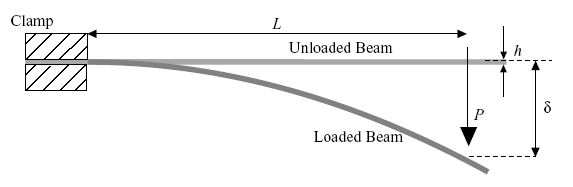
\includegraphics[width=0.7\linewidth]{../Figures/cantilever.png}
\caption{Typical cantilever beam showing length L, concentrated load P and transverse displacement $ \delta $. Graciously borrowed from: \url{http://www.doitpoms.ac.uk/tlplib/thermal-expansion/printall.php}}
\label{fig:cantilever}
\end{figure}


In order to calculate the maximum deflection at the end of a beam of length L, it's useful to know the curvature of the beam:

\begin{equation}\tag{7.1}
\kappa = \frac{M}{EI} = \frac{\partial^2 \delta_{\text{max}}(x)}{\partial x^2}
\end{equation}

Where $ M $ is the concentrated load committing the force upon the beam, $ E $ is the Elastic Modulus and $ I $ is the moment of Inertia.
Solving for $ \delta(x) $ where $ x = L $ gives:

\begin{equation}\tag{7.2}
\delta_{\text{max}}(L) = \frac{PL^3}{3EI}
\end{equation}

Similar equations can be derived for a concentrated load $ P $ at any point along the beam: 

\begin{equation}\tag{7.3}
%\delta_{\text{max}}(x) = \frac{Px^2}{6EI}(3L - x)
\delta_{\text{max}}(x) = \frac{PL^3}{6EI}(3L - x)
\end{equation}

As well as for an uniformly distributed load $ \omega $: 

\begin{equation}\tag{7.4}
\delta_{\text{max}}(\omega) = \frac{\omega L^4}{8EI}
\end{equation}

It is important to note that for the case of the HronTurek Beam with a cross sectional area of $ bh $, the moment of Inertia ($ I $) will be:

\begin{equation}\tag{7.5}
I = \frac{bh^3}{12}
\end{equation}

Where $ h $ is the axis where the bending moment is applied. 

\irsssection{Testing the HronTurek Beam in Elmer}{elmerbeamtest}

Elmer utilizes the finite element method in order to discretize the beam to many sub parts via a mesh. The more nodes the mesh has (in each dimension) the better the approximation, to the analytical solution, will be. There is a trade off of computational time versus accuracy. Understandably, the more dense the mesh, the longer Elmer will take to complete its run. The analytical equations above are only valid once the reduction in error vs. the number of mesh nodes starts to converge.

For this example, it was found that Elmer closely matched the analytical solution once there were: 400 nodes along the length, 16 nodes along the base and 12 nodes along the height of the beam.

A testing script, \textit{HronTurekBeam.csh}, was created to compare the  y-component of the displacement vector of any one Elmer run to the "ideal" case (\textit{yvals\_gold.txt}) within a tolerance of 1.0E-9.

After running the Solver Module Driver (see \irref{Section}{run}), run the HronTurekBeam script in order to make sure your values meet the minimum tolerance. 

\commandline{ctest -R HronTurekBeam}

A text file \textit{yvals\_txt} should be created from the \textit{hronturektest.ep} file created when the \textit{.sif} file is run. From this point the script will diff the \textit{yvals.txt} file against the \textit{yvals\_gold.txt} in order to test for the 1.0E-9 tolerance.

If the test does not pass then the message \textit{"Test data did not pass with tolerance of 1e-9."} will appear. Otherwise, the individual test was successful.
    
\irsection{Troubleshooting}{trouble}

If users encounter problems or have difficulties, please contact us at Illinois Rocstar.

\irwebsite{jkress@illinoisrocstar.com}
